% =============================================================================
% CAPÍTULO 12 — volta 3 (AGENTS.md §6): de onde vem a cauda que as duas explicações usam sem explicar.
%
% O fracasso que o abre, com número na mão: a distância entre o pior e o segundo pior dia, medida
% três vezes, dá três respostas que não se parecem (razões de 1,277 no índice, 1,067 no Ibovespa
% e 1,956 no Bitcoin), e as duas pernas rompem juntas 7,168 vezes o que a independência prevê.
% As duas explicações que sobreviveram à geometria recebem a cauda pronta — nenhuma diz de onde
% ela vem.
%
% Medição: lab/experimentos/E33_cauda.ipynb. Figuras: figuras/E33_cauda_*.
% A assinatura que a aposta inicial esperava — a razão crescer com a amostra no gerador que se
% reproduz — não existe: as três curvas são horizontais. Quem separa é a contagem de recordes: a
% família que se reproduz quebra recordes demais (24 contra 10,48 do harmônico, em vinte mil dias)
% e é refutada nos três mercados; a independente de cauda pesada sobrevive nos três (o t de oito
% graus falha a razão do Bitcoin: 1,956 contra teto de 1,514). Resíduo honesto: os mercados fazem
% menos recordes que o harmônico promete — a porta da lei que anda no tempo.
% =============================================================================

\chapter{De onde vem a cauda}
\label{cap:cauda}

\section{O material que as duas explicações usam}

A volta anterior terminou com duas explicações de pé e uma região estreita para as duas. A troca de
regimes e a persistência sobreviveram a quatro estatísticas porque descrevem \emph{como os dias
ruins se organizam} --- quando vêm, em que ordem, com que constância. Nenhuma das duas diz por que
os dias ruins são \emph{grandes}. As duas recebem a cauda pronta, como quem recebe o material já
cortado, e constroem com ele a sua arrumação. Este capítulo pergunta ao material.

O livro já mediu a cauda três vezes, e as três medidas não se parecem. No índice, o pior dia perde
\numRecordeIndicePior{} contra \numRecordeIndiceSegundo{} do segundo pior --- uma razão de
\numRecordeIndiceRazao{}, distância considerável. No Ibovespa, o pior perde \numRecordeIbovespaPior{}
contra \numRecordeIbovespaSegundo{}: razão de \numRecordeIbovespaRazao{}, quase empatados --- o
pior dia não chega a se destacar do segundo. No Bitcoin, \numRecordeBitcoinPior{} contra
\numRecordeBitcoinSegundo{}: razão de \numRecordeBitcoinRazao{}, o pior dia é o dobro do segundo.
Se a cauda dos três saísse do mesmo mecanismo, a assinatura era uma; são três. E tem o cacho: o
capítulo da queda conjunta mediu as duas pernas rompendo juntas \numConjuntaExcesso{} vezes o que
a independência prevê --- um ajuntamento que nenhuma lei de dias independentes produz, e que
convida a imaginar dias ruins gerando dias ruins.

A pergunta tem forma de gerador. De onde pode ter vindo uma cauda dessas? Há duas histórias
familiares, e este capítulo declara as duas como geradores, para medi-las contra o dado:
a que \textbf{sorteia} --- dias independentes de uma lei de cauda pesada, em que o pior dia é um
sorteio azarado e o seguinte é outro, sem memória entre eles --- e a que \textbf{se reproduz} ---
cada dia ruim gerando dias ruins, a forma de contagio que a literatura da cauda propõe
\cite{dong2020critical}.

\section{As duas famílias declaradas}

A família que sorteia é um \emph{t} de Student com três graus de liberdade, posto na escala de
variância um e multiplicado pela escala do mercado que estiver sendo julgado. Três graus é cauda
que decai devagar --- devagar o bastante para que o pior dia se destaque --- e o capítulo carrega
também o de oito graus, para mostrar que o que vem não depende dessa escolha.

A família que se reproduz é uma ramificação crítica em ambiente aleatório. A cada dia, a população
de dias ruins gera a de amanhã: uma Poisson cuja média é a população de hoje multiplicada pelo
ambiente do dia, e o ambiente é um fator positivo, sem memória entre os dias, com média um --- a
ramificação é crítica em média, nem funeral nem explosão. Extinta a população, um imigrante repõe
um dia ruim no próprio dia: o processo não morre, e a regra está declarada
\cite{dong2020critical}. Um dia ruim com sorte gera descendência demais, a descendência gera a
dele, e o cacho cresce até o ambiente virar. É o gerador que a aposta inicial deste capítulo
favorecia: nele, os dias grandes chegam juntos porque um gerou o outro.

As duas famílias foram calibradas pela mesma regra, e a regra é declarada: cada mundo sai em
unidades de desvio-padrão e é multiplicado pela escala do mercado. As assinaturas medidas --- a
razão entre o pior e o segundo pior dia, a contagem de recordes --- não dependem da escala, e é
por isso que a calibração pode se dar por ela. A medição usa \numCaudaMundos{} mundos por família
no tamanho de amostra de cada mercado, \numCaudaMundosCurva{} por ponto das curvas, e o número que
alimenta o sorteador é o mesmo em todo o caderno: \numCaudaSemente{}.

\section{A assinatura que não existe}

A aposta inicial era explícita: se o pior dia é um sorteio solto, a razão entre os dois piores não
depende de quantos dias se olhou; se os dias grandes vêm de cacho, olhar mais dias acha cachos
maiores, e a razão cresce com a amostra. A assinatura separaria as histórias sem precisar ajustar
nada.

Ela não existe. Medida de duzentos e cinquenta a vinte mil dias, a razão mediana do \emph{t} de
três graus vai de \numCaudaIndependenteRazaoInicio{} a \numCaudaIndependenteRazaoFim{}; a do de
oito graus, de \numCaudaIndependenteOitoRazaoInicio{} a \numCaudaIndependenteOitoRazaoFim{}; a da
ramificação crítica, de \numCaudaReproducaoRazaoInicio{} a \numCaudaReproducaoRazaoFim{}. As três
curvas são horizontais (Figura~\ref{fig:cauda-curvas}, esquerda). Olhar oitenta vezes mais dias
não afasta o segundo pior do primeiro --- em nenhuma das duas famílias.

A razão entre extremos é evidência fraca, e o desenho mostra por quê: as nuvens de mundos têm
rabos direitos longos, mundos em que o segundo pior veio pequeno demais e a razão explode. Amostrar
extremos é amostrar cauda, e cauda se amostra mal --- o mesmo aviso que a estimativa sob variância
infinita dá ao resto da estatística \cite{fontanari2020gini}. Uma assinatura que era para separar
famílias separa quase nada: a informação está em outro lugar.

\section{Quem quebra recordes}

Está no tempo. Um dia que supera todos os anteriores --- um recorde --- deixa uma contagem, e a
contagem tem uma promessa exata para dias independentes: o número esperado de novas marcas em
\emph{n} dias é o harmônico, que cresce como o logaritmo. A promessa é livre de distribuição: não
importa a lei dos dias, contanto que sejam independentes e trocáveis. Duas leis de cauda
diferentes prometem o mesmo número de marcas --- e um gerador de cachos, não.

% aterramento: recorde
As duas famílias do \emph{t} cumprem a promessa: a mediana da contagem vai de
\numCaudaIndependenteRecordesInicio{} em duzentos e cinquenta dias a \numCaudaIndependenteRecordesFim{}
em vinte mil, com o harmônico indo de \numCaudaRecordesEsperadoInicio{} a
\numCaudaIndependenteRecordesEsperadoFim{}. A ramificação crítica sai de junto da promessa e sobe
sozinha: de \numCaudaReproducaoRecordesInicio{} a \numCaudaReproducaoRecordesFim{}
(Figura~\ref{fig:cauda-curvas}, direita). O dobro da promessa, e é fácil ver por quê: cada cacho
que passa tudo o que veio antes quebra a marca várias vezes na subida --- o gerador que concentrava
a cauda em episódios paga isso em marcas, uma atrás da outra.

A assinatura que a razão não entregou, a contagem entregou --- ao contrário da aposta: o gerador
que se reproduz não se limita a fazer cachos grandes, ele faz marcas demais.

\section{A decisão, mercado por mercado}

O critério é o declarado no começo: no tamanho de amostra do próprio mercado, \numCaudaMundos{}
mundos por família na escala do mercado, e a família reproduz o mercado quando o ponto dele --- a
razão e a contagem --- cai dentro dos percentis cinco a noventa e cinco da nuvem, nas duas
margens. A Tabela~\ref{tab:cauda-decisao} mostra as duas famílias que restam --- o \emph{t} de
três graus e a ramificação crítica; o de oito entra na prosa, porque falha logo.

\begin{table}[htbp]
\centering
\resizebox{\linewidth}{!}{%
\begin{tabular}{@{}lrrrr@{}}
    \hline
 & razão (med.) & razão (faixa) & marcas (med.) & marcas (faixa) \\
    \hline
índice, sorteia & \numCaudaNuvemSpIndependenteRazaoMediana{} & \numCaudaNuvemSpIndependenteRazaoPiso{}--\numCaudaNuvemSpIndependenteRazaoTeto{} & \numCaudaNuvemSpIndependenteRecordesMediana{} & \numCaudaNuvemSpIndependenteRecordesPiso{}--\numCaudaNuvemSpIndependenteRecordesTeto{} \\
índice, reproduz & \numCaudaNuvemSpReproducaoRazaoMediana{} & \numCaudaNuvemSpReproducaoRazaoPiso{}--\numCaudaNuvemSpReproducaoRazaoTeto{} & \numCaudaNuvemSpReproducaoRecordesMediana{} & \numCaudaNuvemSpReproducaoRecordesPiso{}--\numCaudaNuvemSpReproducaoRecordesTeto{} \\
Ibovespa, sorteia & \numCaudaNuvemIbovIndependenteRazaoMediana{} & \numCaudaNuvemIbovIndependenteRazaoPiso{}--\numCaudaNuvemIbovIndependenteRazaoTeto{} & \numCaudaNuvemIbovIndependenteRecordesMediana{} & \numCaudaNuvemIbovIndependenteRecordesPiso{}--\numCaudaNuvemIbovIndependenteRecordesTeto{} \\
Ibovespa, reproduz & \numCaudaNuvemIbovReproducaoRazaoMediana{} & \numCaudaNuvemIbovReproducaoRazaoPiso{}--\numCaudaNuvemIbovReproducaoRazaoTeto{} & \numCaudaNuvemIbovReproducaoRecordesMediana{} & \numCaudaNuvemIbovReproducaoRecordesPiso{}--\numCaudaNuvemIbovReproducaoRecordesTeto{} \\
Bitcoin, sorteia & \numCaudaNuvemBtcIndependenteRazaoMediana{} & \numCaudaNuvemBtcIndependenteRazaoPiso{}--\numCaudaNuvemBtcIndependenteRazaoTeto{} & \numCaudaNuvemBtcIndependenteRecordesMediana{} & \numCaudaNuvemBtcIndependenteRecordesPiso{}--\numCaudaNuvemBtcIndependenteRecordesTeto{} \\
Bitcoin, reproduz & \numCaudaNuvemBtcReproducaoRazaoMediana{} & \numCaudaNuvemBtcReproducaoRazaoPiso{}--\numCaudaNuvemBtcReproducaoRazaoTeto{} & \numCaudaNuvemBtcReproducaoRecordesMediana{} & \numCaudaNuvemBtcReproducaoRecordesPiso{}--\numCaudaNuvemBtcReproducaoRecordesTeto{} \\
    \hline
\end{tabular}}
\caption{A decisão, mercado por mercado: razão entre os dois piores dias e contagem de marcas
(mediana e faixa de cinco a noventa e cinco por cento) na nuvem de \numCaudaMundos{} mundos de
cada família, no tamanho de amostra de cada mercado. Os mercados fazem \numCaudaSpRecordes{},
\numCaudaIbovRecordes{} e \numCaudaBtcRecordes{} marcas, contra promessas de \numCaudaSpEsperado{},
\numCaudaIbovEsperado{} e \numCaudaBtcEsperado{}.}
\label{tab:cauda-decisao}
\end{table}

\begin{figure}[htbp]
\centering
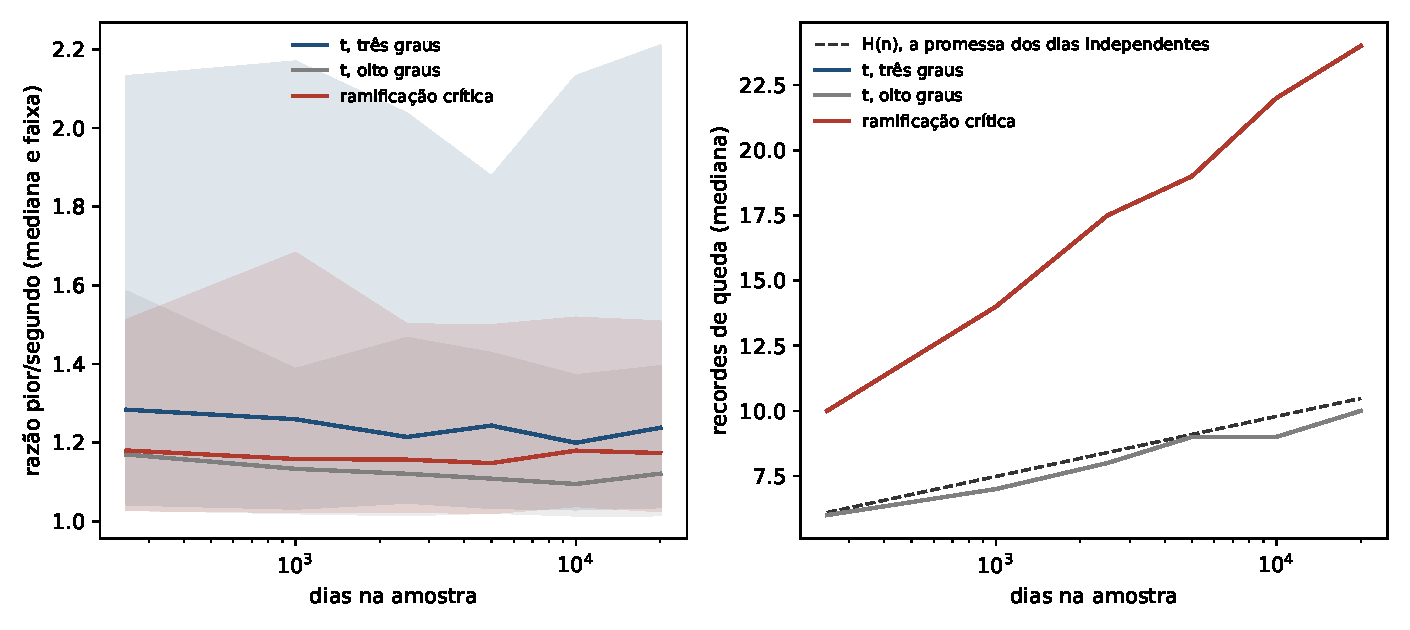
\includegraphics[width=\textwidth]{figuras/E33_cauda_1.pdf}
\caption{A razão entre os dois piores dias (esquerda) e a contagem de marcas (direita), contra o
tamanho da amostra, em mediana e faixa: o \emph{t} de três graus em azul, o de oito em cinza, a
ramificação crítica em vermelho, e o harmônico tracejado --- a promessa dos dias independentes. As
três curvas da esquerda são horizontais; na direita, as duas do \emph{t} andam coladas no tracejado
e a da ramificação sobe sozinha para o dobro.}
\label{fig:cauda-curvas}
\end{figure}

\begin{figure}[htbp]
\centering
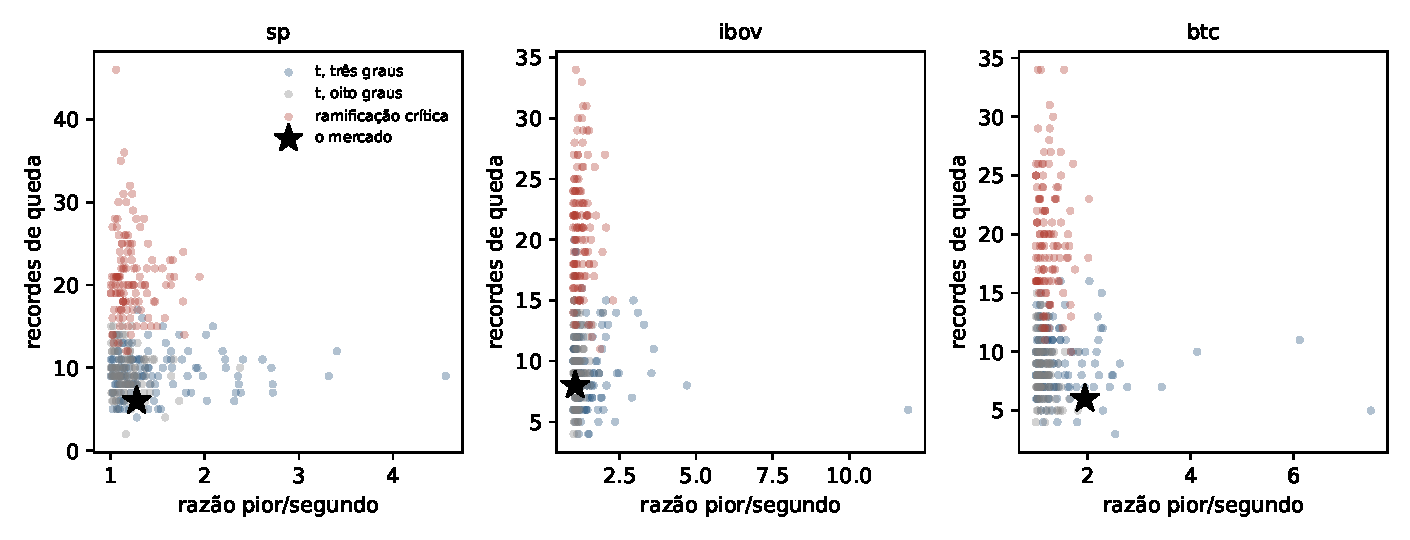
\includegraphics[width=\textwidth]{figuras/E33_cauda_2.pdf}
\caption{A decisão: a nuvem de mundos de cada família (a razão contra a contagem de marcas) e a
estrela do mercado, nos três painéis. As estrelas caem na parte baixa das nuvens do \emph{t} e
sempre abaixo das nuvens da ramificação, que moram acima das marcas que os mercados fazem. No
Bitcoin, a estrela está à direita da nuvem cinza --- o \emph{t} de oito graus não faz razão de
\numRecordeBitcoinRazao{}: o teto dele é \numCaudaNuvemBtcIndependenteOitoRazaoTeto{}.}
\label{fig:cauda-decisao}
\end{figure}

O \emph{t} de três graus reproduz os três mercados: as razões do índice, do Ibovespa e do Bitcoin
cabem nas faixas dele, e as contagens também. O de oito graus reprova no Bitcoin --- a razão de
\numRecordeBitcoinRazao{} passa o teto de \numCaudaNuvemBtcIndependenteOitoRazaoTeto{} --- e
aprova nos outros dois: a cauda tem de ser pesada de verdade para o mercado que mais distancia o
pior do segundo, e grau a mais não é um detalhe. A ramificação crítica reprova nos três, e sempre
pela mesma margem: as contagens. Os mercados fazem \numCaudaSpRecordes{}, \numCaudaIbovRecordes{}
e \numCaudaBtcRecordes{} marcas; as nuvens da ramificação começam em
\numCaudaNuvemSpReproducaoRecordesPiso{} no índice --- e as do Ibovespa e do Bitcoin, acima disso.
O gerador que se reproduz não é rejeitado por fazer cauda curta: é rejeitado por fazer marcas
demais.

E as contagens dos próprios mercados carregam um aviso que nenhuma das duas famílias atende: a
promessa dos dias independentes é de \numCaudaSpEsperado{} marcas no índice, e ele fez
\numCaudaSpRecordes{}; \numCaudaIbovEsperado{} no Ibovespa, que fez \numCaudaIbovRecordes{};
\numCaudaBtcEsperado{} no Bitcoin, que fez \numCaudaBtcRecordes{}. Os três ficaram abaixo ---
dentro da faixa do \emph{t}, mas na parte baixa, e sempre do mesmo lado. Poucas marcas querem
dizer extremos cedo: os maiores dias destas séries vieram nos primeiros anos, e o resto do
registro não conseguiu superá-los. Dia independente nenhum prefere o começo --- nenhuma lei
estável prefere. É o resíduo deste capítulo, e ele tem dono: uma lei que anda no tempo.

\section{O que fica}

Fica a pergunta respondida com a forma honesta que ela aceita: destes três mercados, a cauda
convive com dias independentes de lei pesada --- o gerador mais simples que se oferecia passou no
teste que os outros reprovaram --- e não convive com o mecanismo que se reproduz, que a intuição
do cacho recomendava. A intuição não era burra: o cacho existe, o capítulo da queda conjunta
mediu-o de novo aqui na abertura. Mas existe \emph{entre} pernas --- um mercado caindo junto com o
outro ---, e a medição deste capítulo é sobre o tempo \emph{dentro} de um mercado só. A dependência
entre margens e a reprodução no tempo são histórias diferentes, e a segunda, sozinha, não sustenta
os dados: é o tipo de correção que só aparece quando as duas são declaradas como geradores e
medidas separadas.

Fica o método: a assinatura que devia separar (a razão crescente) não existia, e a que separava
estava em outro lugar (as marcas); um capítulo que fosse escrito na aposta inicial teria dito o
contrário do que a medição disse. E fica o instrumento novo no cinto: a contagem de marcas, com a
sua promessa livre de distribuição, que o resto do livro ainda vai usar.

E fica o resíduo, que é uma porta: os extremos vieram cedo, a lei não é estável, os parâmetros
andam. Interrogou-se o material, e ele respondeu --- com uma direção. A pergunta que a volta
anterior deixou adiada pode voltar agora com o material esclarecido: se ver mais mundos basta para
escolher entre as duas explicações que sobreviveram, ou se é preciso mexer no mundo de propósito.
É essa a pergunta seguinte.
